\section{Wireless Bottleneck Detector}\label{Wireless Bottleneck Detector}

In this section we describe the tool we have created.

It is a \emph{custom} version of Ping in \emph{GoLang}. This custom version allow us to define a probing rate, send probes in batches and set an inter-space between probes and batches.

Explain we have used exponential distribution to send batches. We have chosen exponential as Poisson process is related to exponential arrival times. We chose Poisson because sampling a Poisson process results in Poisson process, which allows to keep the same Poisson process even after sampling.

The sampling technique we used is Bernoulli, which is a type of Poisson sampling. In Bernoulli sampling all the observation in the data set have the same probability to become or not to become part of the resulting sampling set.

We varied the probability to be part of the sampling from 10\% to 90\%. To choose the sample which resembles the most to our original data set we worked with \emph{Two Sample Kolmogorov-Smirnov} Test
\\
\\
\textbf{Main characteristics of Ping Tool.}
\begin{itemize}
	\item The ping tool being used has been customized to be able to send batches of pings.
	\item The tool allows to define a probing rate based on a Poisson process, exponential distribution. We have chosen a Poisson process as we sample from it. Sampling from a Poisson process leads to another Poisson process.
	\item Our sampling rate has been defined to be 200 msec based on sampling and similarity test results.
\end{itemize}

Based on the similarity test conducted the rate at which batches will be sent has been defined to 200msec. Each 200msec a batch of 3 pings will be send, from the 3rd ping we will extract the RTT. We have chosen the 3rd ping as we found to be the one preventing the case of sleeping NIC, the first two ping were experiencing higher RTT due to sleeping NIC case. We tested this case in our lab by disabling power save mode in the Wireless NIC and noticing RTT went down for the first two pings. The case of sleeping NIC is often avoided with ping rate lower than 100msec, i.e. 90, 80, 50 msec. To validate our sampling rate, 200msec still holds in our testbed we conducted tests. The tests consisted in sending as many batches as possible for 10 min at 100 and 200msec. Additionally we varied the attenuation from 0, 15 and 30 dBm. The test sessions were conducted in the 2.4 GHz band using and 802.11n WLAN with no authentication. Each of the experiments was conducted 5 times, in total we obtained 30 samples.

\begin{center}
	\begin{tabular}{||c c||}
		\hline
		Attenuation & Rate\\ [0.5ex] 
		\hline\hline
		0 dBm & 100msec\\ 
		\hline
		0 dBm & 200msec\\
		\hline
		15 dBm & 100msec\\
		\hline
		15 dBm & 200msec\\
		\hline
		30 dBm & 100msec\\
		\hline
		30 dBm & 200msec\\ [1ex] 
		\hline
	\end{tabular}
\end{center}

To validate the similarity between the rates we compared the ECDF of each one, the curves must resemble to each other. In our case the results between 100 and 200 msec rate are depicted in the following images. In figure \ref{att_0_100and200msec} it can be perceived similarity between two rates.

\begin{figure}[h]
	\centering
	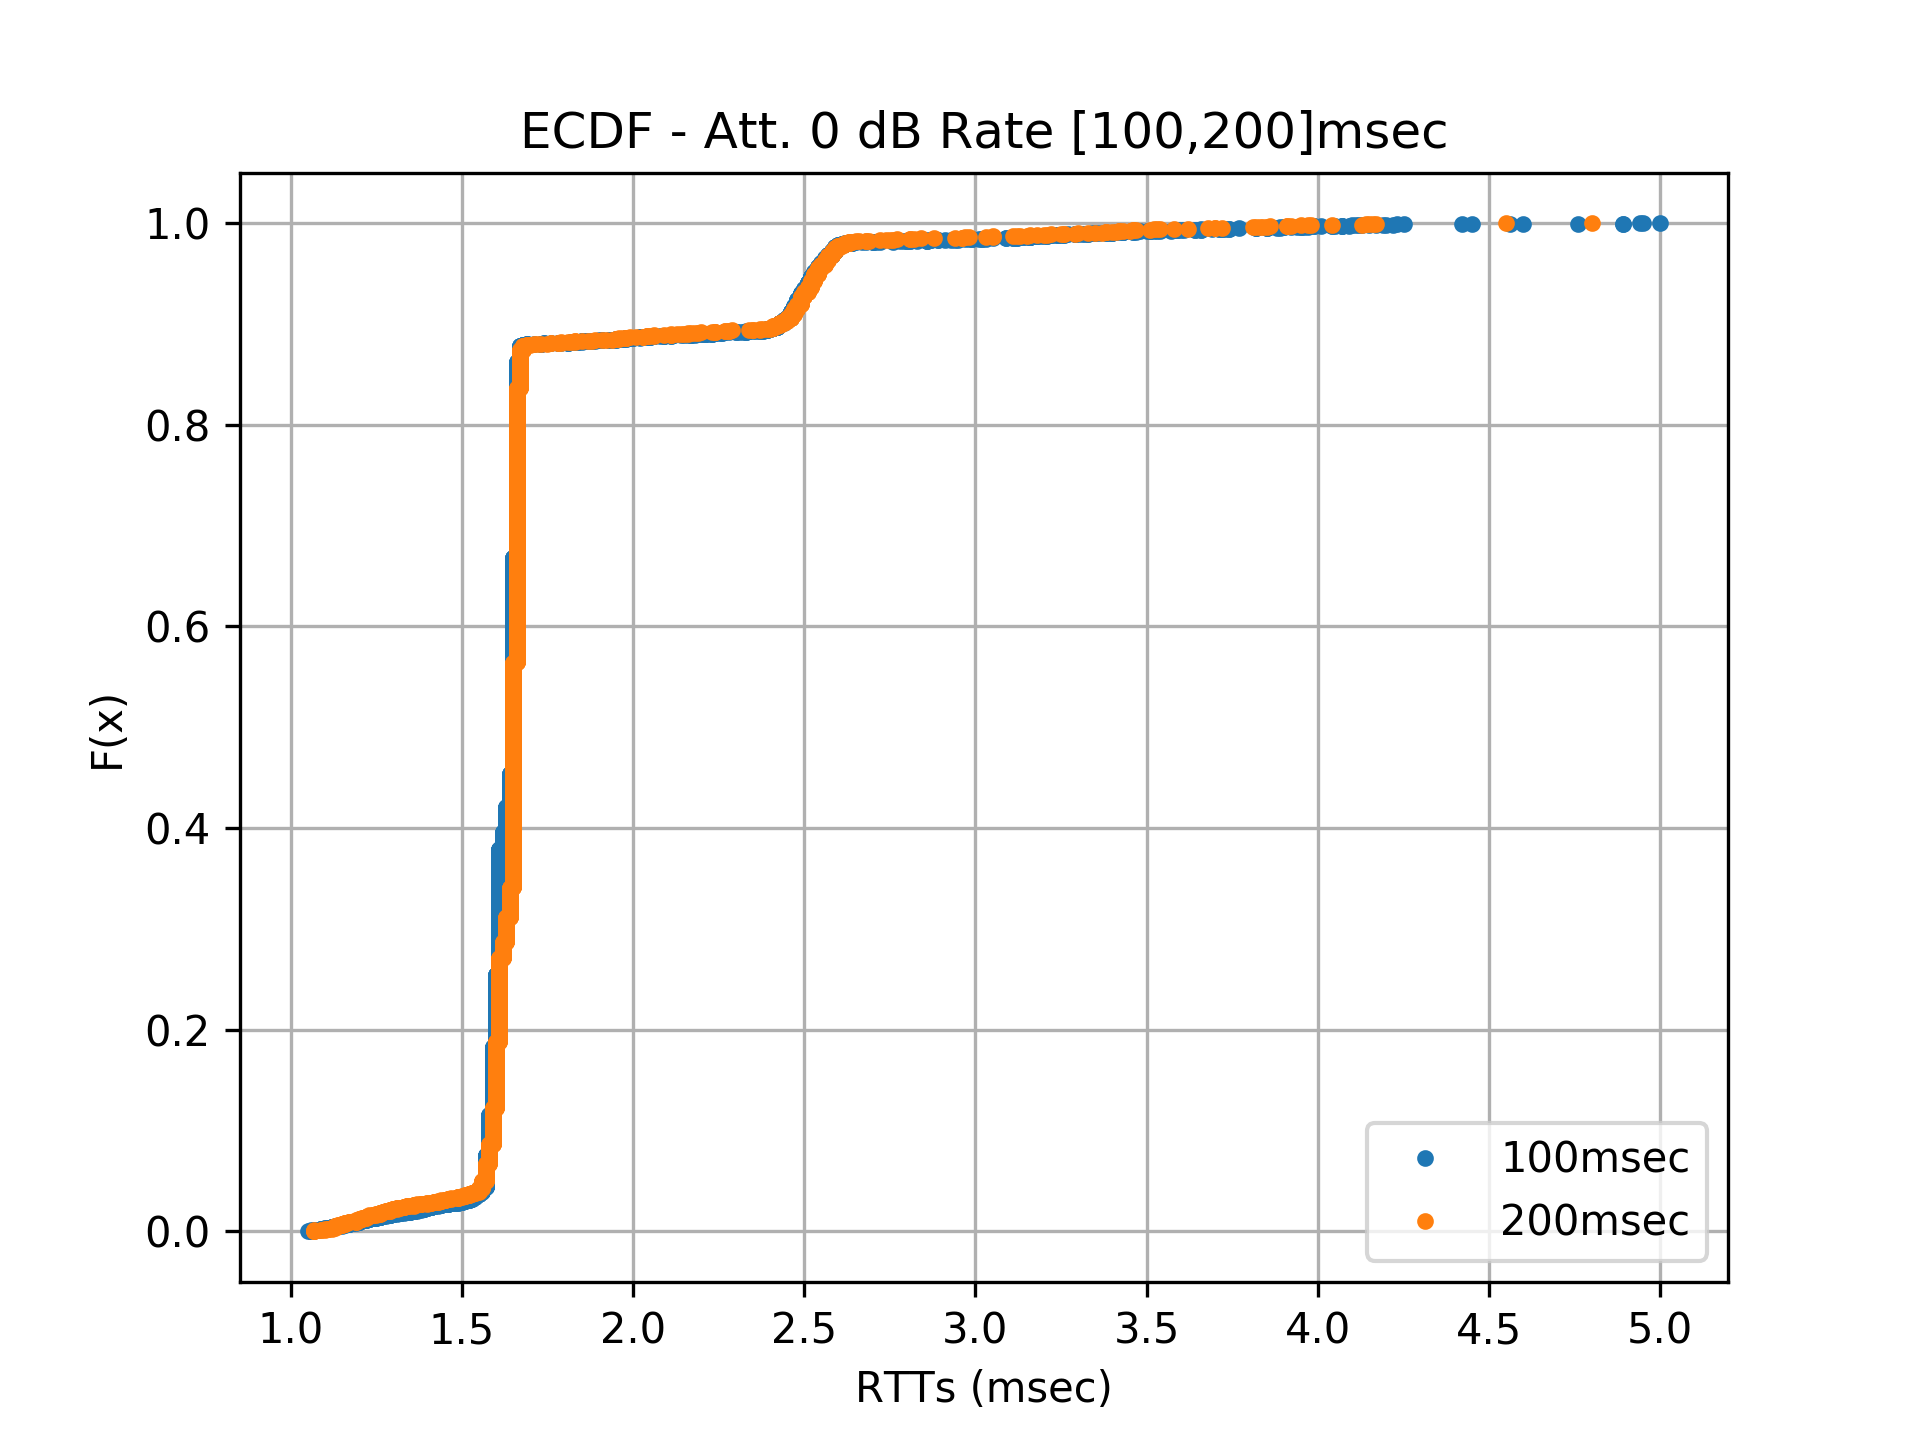
\includegraphics[width=8cm]{Rates_Atts/Att_0dBRate[100,200]msec}
	\caption{Att. 0 dBm - Rate 100,200 msec}
	\label{att_0_100and200msec}
\end{figure}

Figure \ref{rate_200msec_Att_0_15_30dBm} help us to validate an expected behavior. As we increase attenuation, the RTT is expected to be higher. This behavior is depicted in figure \ref{rate_200msec_Att_0_15_30dBm}.

\begin{figure}[h]
	\centering
	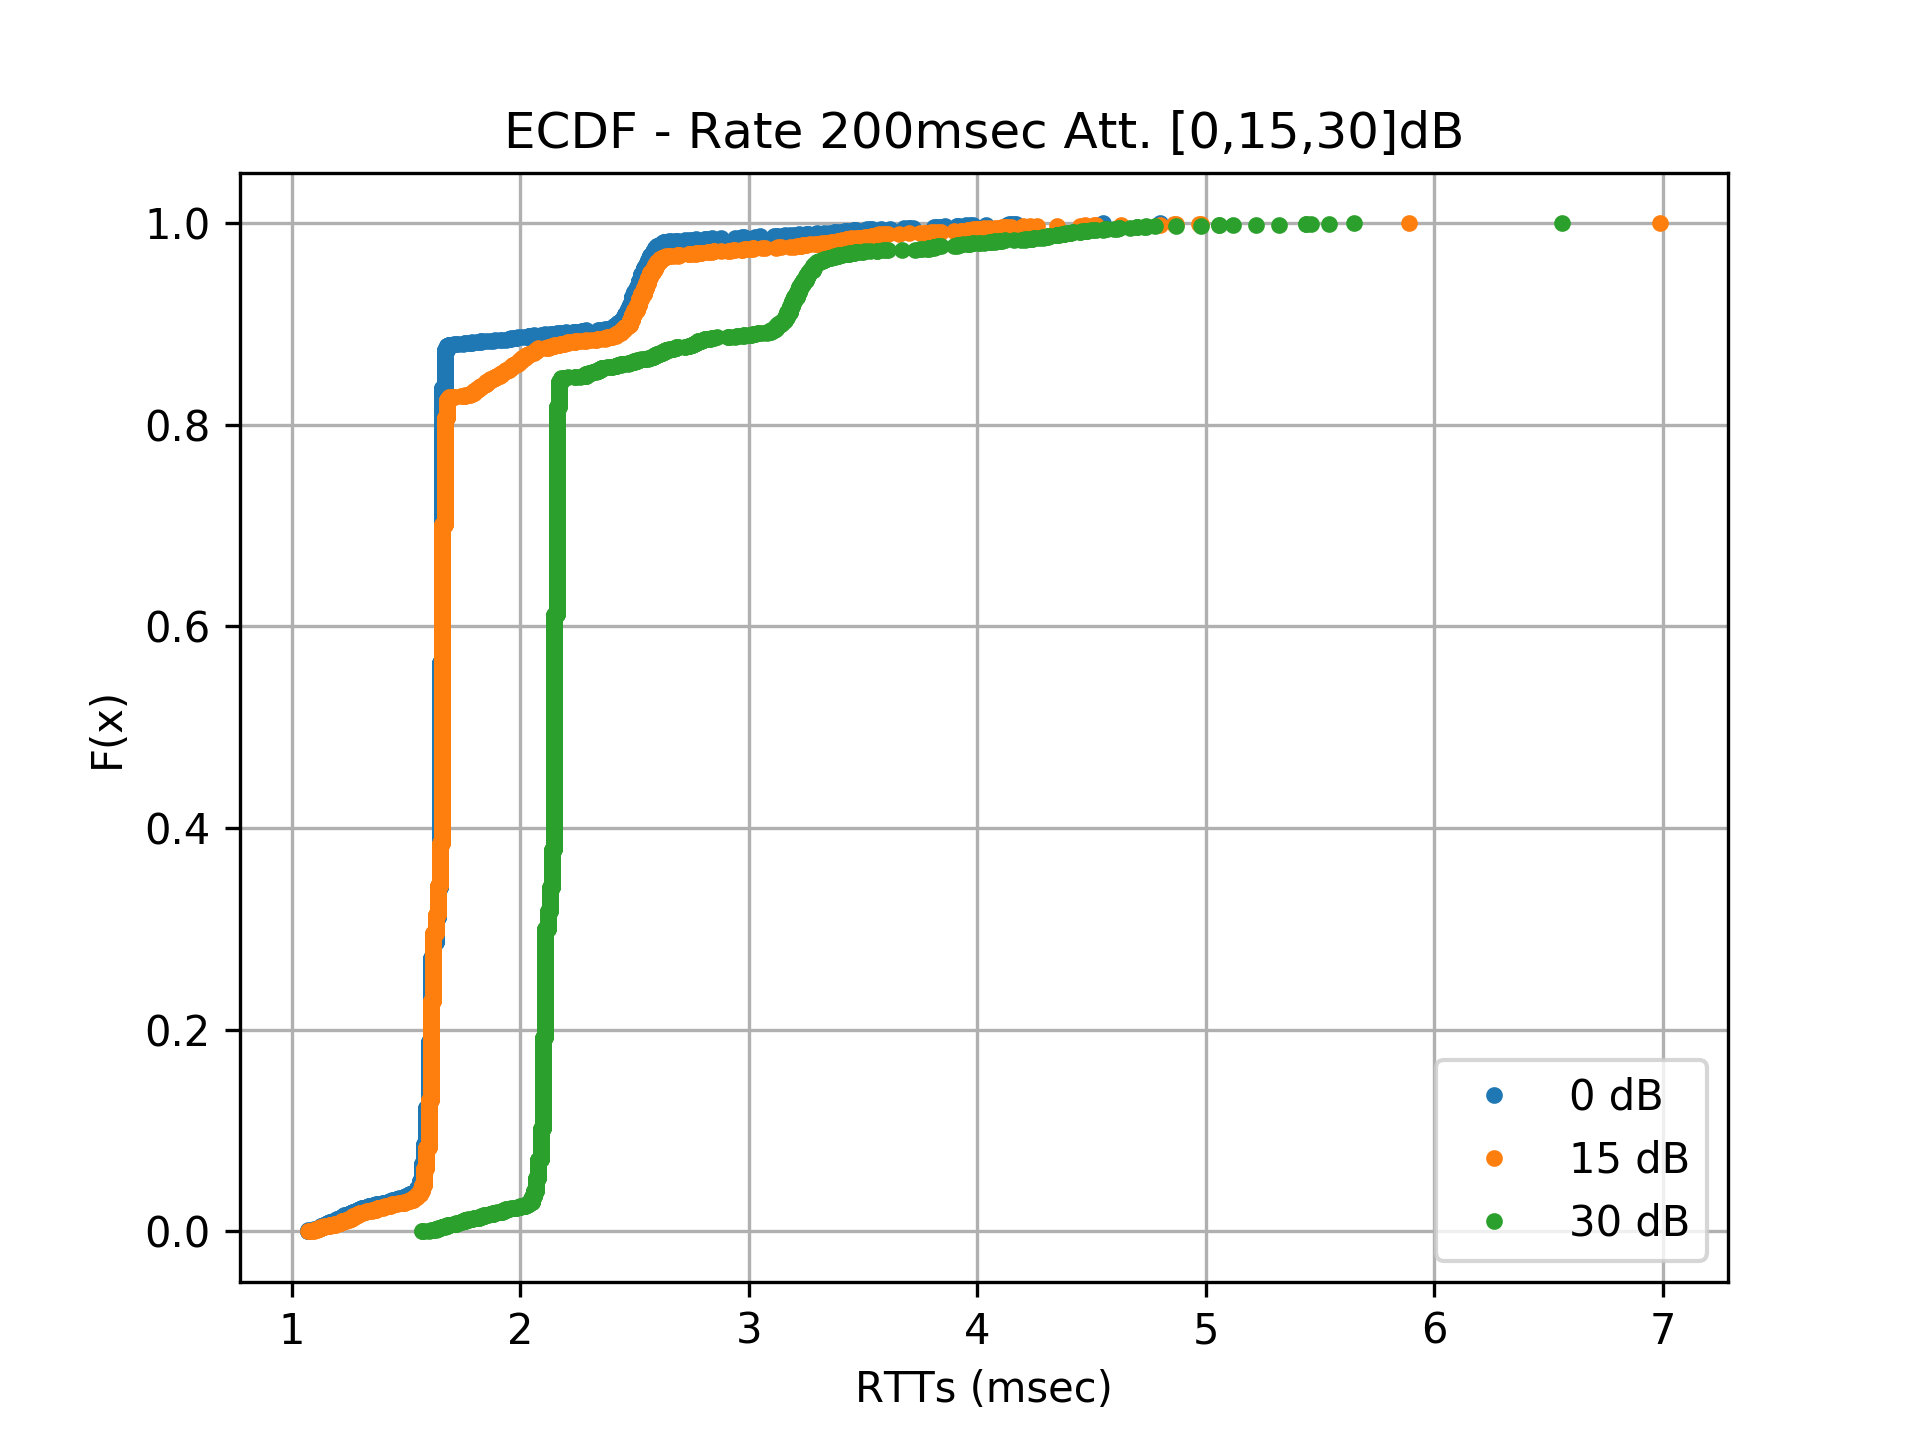
\includegraphics[width=8cm]{Rates_Atts/Rate200msecAtt_[0,15,30]dB}
	\caption{Rate 200 msec - Att. [0,15,30] dB}
	\label{rate_200msec_Att_0_15_30dBm}
\end{figure}

\emph{We can also describe that the p-value is close to 1 and the D-Value, which is the KS statistic is low. KS Low value is pursed as it means distance between the two ECDFs is small, meaning they are close to each other, hence more similar.}